% ============================================================
% 第23章 旋转 — 人教版九年级上册
% 编译命令：xelatex -interaction=nonstopmode 第23章_旋转.tex
% ============================================================
\documentclass[12pt, a4paper]{ctexart}
\usepackage[margin=2.2cm]{geometry}
\usepackage{amsmath, amssymb}
\usepackage{enumitem}
\usepackage{tcolorbox}
\usepackage{booktabs}
\usepackage{array}
\usepackage{fancyhdr}
\usepackage{xcolor}
\usepackage{tikz}
\usepackage{hyperref}
\usepackage{graphicx}
\usepackage{multirow}
\usepackage{pgfplots}
\pgfplotsset{compat=1.18}

% 颜色定义
\definecolor{mainblue}{RGB}{41, 98, 168}
\definecolor{lightblue}{RGB}{230, 240, 255}
\definecolor{tipgreen}{RGB}{34, 139, 87}
\definecolor{lightgreen}{RGB}{235, 250, 240}
\definecolor{warnred}{RGB}{200, 50, 50}
\definecolor{lightred}{RGB}{255, 240, 240}
\definecolor{examorange}{RGB}{210, 120, 20}
\definecolor{lightorange}{RGB}{255, 248, 235}
\definecolor{apppurple}{RGB}{120, 60, 170}
\definecolor{lightpurple}{RGB}{245, 238, 255}

% 页眉页脚
\pagestyle{fancy}
\fancyhf{}
\fancyhead[L]{\small\textcolor{mainblue}{\textbf{人教版九年级上册 \(\cdot\) 第23章 旋转}}}
\fancyhead[R]{\small\textcolor{mainblue}{家教讲义}}
\fancyfoot[C]{\small —\ \thepage\ —}
\renewcommand{\headrulewidth}{0.6pt}
\renewcommand{\headrule}{\hbox to\headwidth{\color{mainblue}\leaders\hrule height \headrulewidth\hfill}}
\renewcommand{\footrulewidth}{0pt}

% tcolorbox 样式
\newtcolorbox{knowledgebox}[1][]{%
  colback=lightblue, colframe=mainblue,
  fonttitle=\bfseries\large, title=#1,
  arc=3mm, boxrule=0.8pt,
  left=8pt, right=8pt, top=6pt, bottom=6pt
}

\newtcolorbox{tipbox}[1][]{%
  colback=lightgreen, colframe=tipgreen,
  fonttitle=\bfseries, title=#1,
  arc=2mm, boxrule=0.6pt,
  left=6pt, right=6pt, top=4pt, bottom=4pt
}

\newtcolorbox{warnbox}[1][]{%
  colback=lightred, colframe=warnred,
  fonttitle=\bfseries, title=#1,
  arc=2mm, boxrule=0.6pt,
  left=6pt, right=6pt, top=4pt, bottom=4pt
}

\newtcolorbox{examplebox}[1][]{%
  colback=lightorange, colframe=examorange,
  fonttitle=\bfseries, title=#1,
  arc=3mm, boxrule=0.8pt,
  left=8pt, right=8pt, top=6pt, bottom=6pt
}

\newtcolorbox{appbox}[1][]{%
  colback=lightpurple, colframe=apppurple,
  fonttitle=\bfseries, title=#1,
  arc=3mm, boxrule=0.8pt,
  left=8pt, right=8pt, top=6pt, bottom=6pt
}

\setCJKmainfont{Hiragino Sans GB}
\setCJKsansfont{Heiti SC}

\begin{document}

% ============ 标题页 ============
\begin{center}
{\Huge\bfseries\textcolor{mainblue}{第23章\quad 旋\ 转}}\\[12pt]
{\Large\textcolor{gray}{家\ 教\ 讲\ 义}}\\[8pt]
\rule{0.6\textwidth}{1pt}\\[8pt]
{\normalsize 适用：人教版\quad 九年级上册\quad |\quad 课时：4课时}
\end{center}
\vspace{10pt}

% ==============================================================
% 第一部分：知识点讲解
% ==============================================================
\section*{\textcolor{mainblue}{一、知识点讲解}}

% -------------------- 23.1 旋转 --------------------
\subsection*{23.1\quad 旋转的概念}

\begin{knowledgebox}[旋转的定义]
把一个平面图形绕着平面内某一个点 $O$ 转动一个角度，叫做图形的\textbf{旋转}。点 $O$ 叫做\textbf{旋转中心}，转动的角叫做\textbf{旋转角}。

如果图形上的点 $P$ 经过旋转变为点 $P'$，那么这两个点叫做这个旋转的\textbf{对应点}。
\end{knowledgebox}

\begin{knowledgebox}[旋转的三要素]
旋转由以下三个要素唯一确定：
\begin{enumerate}[nosep]
  \item \textbf{旋转中心}——绕哪个点旋转；
  \item \textbf{旋转方向}——顺时针还是逆时针；
  \item \textbf{旋转角度}——转动了多少度。
\end{enumerate}
三者缺一不可，改变其中任何一个，旋转的结果都会不同。
\end{knowledgebox}

\begin{center}
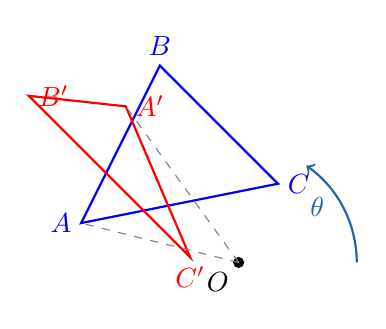
\begin{tikzpicture}[scale=1.0]
  % 旋转中心
  \fill (0,0) circle (2pt) node[below left]{$O$};
  % 原三角形 ABC
  \coordinate (A) at (-2, 0.5);
  \coordinate (B) at (-1, 2.5);
  \coordinate (C) at (0.5, 1);
  \draw[thick, blue] (A) -- (B) -- (C) -- cycle;
  \node[left, blue] at (A) {$A$};
  \node[above, blue] at (B) {$B$};
  \node[right, blue] at (C) {$C$};
  % 旋转后的三角形 A'B'C' (逆时针旋转60度)
  \coordinate (Ap) at ({-2*cos(60)-0.5*sin(60)}, {-2*(-sin(60))+0.5*cos(60)});
  \coordinate (Bp) at ({-1*cos(60)-2.5*sin(60)}, {-1*(-sin(60))+2.5*cos(60)});
  \coordinate (Cp) at ({0.5*cos(60)-1*sin(60)}, {0.5*(-sin(60))+1*cos(60)});
  \draw[thick, red] (Ap) -- (Bp) -- (Cp) -- cycle;
  \node[right, red] at (Ap) {$A'$};
  \node[right, red] at (Bp) {$B'$};
  \node[below, red] at (Cp) {$C'$};
  % 旋转角弧线
  \draw[->, thick, mainblue] (1.5, 0) arc (0:55:1.5);
  \node[mainblue] at (1.0, 0.7) {$\theta$};
  % OA, OA'
  \draw[dashed, gray] (0,0) -- (A);
  \draw[dashed, gray] (0,0) -- (Ap);
\end{tikzpicture}
\end{center}

% -------------------- 23.2 旋转的性质 --------------------
\subsection*{23.2\quad 旋转的性质}

\begin{knowledgebox}[旋转的性质]
旋转具有以下重要性质：
\begin{enumerate}[nosep]
  \item 对应点到旋转中心的距离\textbf{相等}。即 $OA = OA'$，$OB = OB'$，$OC = OC'$。
  \item 每对对应点与旋转中心所连线段的夹角都等于\textbf{旋转角}。即 $\angle AOA' = \angle BOB' = \angle COC' = \theta$。
  \item 旋转前后的图形\textbf{全等}（对应线段相等、对应角相等）。
\end{enumerate}
\end{knowledgebox}

\begin{center}
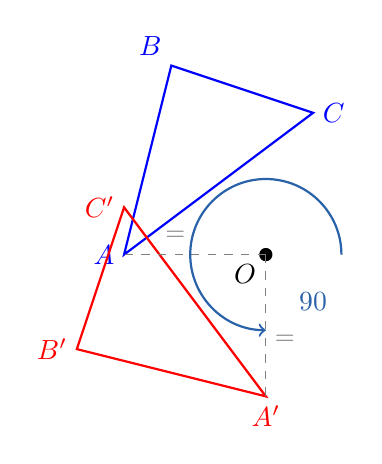
\begin{tikzpicture}[scale=1.2]
  % 旋转中心
  \fill (0,0) circle (2pt) node[below left]{$O$};
  % 原三角形
  \coordinate (A) at (-1.5, 0);
  \coordinate (B) at (-1, 2);
  \coordinate (C) at (0.5, 1.5);
  \draw[thick, blue] (A) -- (B) -- (C) -- cycle;
  \node[left, blue] at (A) {$A$};
  \node[above left, blue] at (B) {$B$};
  \node[right, blue] at (C) {$C$};
  % 旋转90度后的三角形
  \coordinate (Ap) at (0, -1.5);
  \coordinate (Bp) at (-2, -1);
  \coordinate (Cp) at (-1.5, 0.5);
  \draw[thick, red] (Ap) -- (Bp) -- (Cp) -- cycle;
  \node[below, red] at (Ap) {$A'$};
  \node[left, red] at (Bp) {$B'$};
  \node[left, red] at (Cp) {$C'$};
  % OA = OA'
  \draw[dashed, gray] (0,0) -- (A);
  \draw[dashed, gray] (0,0) -- (Ap);
  \node[left, font=\small, gray] at (-0.75, 0.2) {$=$};
  \node[below, font=\small, gray] at (0.2, -0.75) {$=$};
  % 旋转角
  \draw[->, thick, mainblue] (0.8, 0) arc (0:270:0.8);
  \node[mainblue] at (0.5, -0.5) {$90°$};
\end{tikzpicture}
\end{center}

\begin{warnbox}[易错提醒]
\begin{enumerate}[nosep]
  \item 旋转不改变图形的\textbf{形状}和\textbf{大小}，只改变图形的\textbf{位置}。
  \item "对应点到旋转中心距离相等"意味着旋转中心在对应点连线段的\textbf{垂直平分线}上。
  \item 旋转角不一定是锐角，可以是任意角度（如 $180°$、$270°$ 等）。
  \item 注意区分"旋转方向"：顺时针旋转与逆时针旋转的结果不同。
\end{enumerate}
\end{warnbox}

% -------------------- 23.3 旋转作图 --------------------
\subsection*{23.3\quad 旋转作图}

\begin{knowledgebox}[旋转作图的步骤]
将图形绕某点旋转指定角度的步骤：
\begin{enumerate}[nosep]
  \item 确定\textbf{旋转中心} $O$、\textbf{旋转方向}和\textbf{旋转角} $\theta$。
  \item 将图形的每个关键点分别与旋转中心 $O$ 连接。
  \item 以旋转中心为顶点，分别以各连线为一边，按指定方向作角等于 $\theta$。
  \item 在所作角的另一边上截取对应线段，使对应点到旋转中心的距离等于原对应点到旋转中心的距离。
  \item 顺次连接各对应点，得到旋转后的图形。
\end{enumerate}
\end{knowledgebox}

\begin{tipbox}[旋转作图的关键]
旋转作图的核心是"定点旋转"——将图形的每个顶点分别绕旋转中心旋转相同的角度和方向，然后连接新的顶点。实际操作中常用圆规截取等距，用量角器度量旋转角。
\end{tipbox}

% -------------------- 23.4 中心对称 --------------------
\subsection*{23.4\quad 中心对称}

\begin{knowledgebox}[中心对称的定义]
把一个图形绕着某一个点旋转 $180°$，如果它能够与另一个图形重合，那么就说这两个图形\textbf{关于这个点对称}（即\textbf{中心对称}）。这个点叫做\textbf{对称中心}。

中心对称是旋转角为 $180°$ 的特殊旋转。
\end{knowledgebox}

\begin{center}
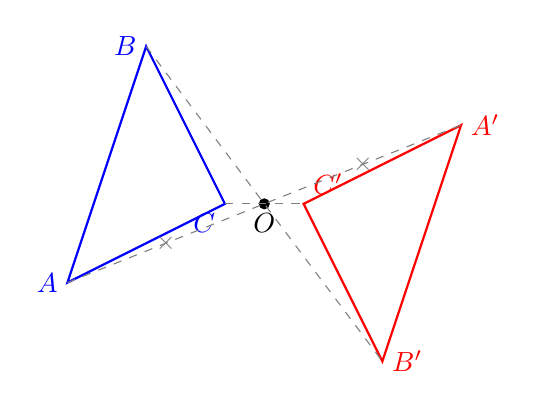
\begin{tikzpicture}[scale=1.0]
  % 对称中心
  \fill (0,0) circle (2pt) node[below]{$O$};
  % 左侧三角形
  \coordinate (A) at (-2.5, -1);
  \coordinate (B) at (-1.5, 2);
  \coordinate (C) at (-0.5, 0);
  \draw[thick, blue] (A) -- (B) -- (C) -- cycle;
  \node[left, blue] at (A) {$A$};
  \node[left, blue] at (B) {$B$};
  \node[below left, blue] at (C) {$C$};
  % 右侧三角形（旋转180度）
  \coordinate (Ap) at (2.5, 1);
  \coordinate (Bp) at (1.5, -2);
  \coordinate (Cp) at (0.5, 0);
  \draw[thick, red] (Ap) -- (Bp) -- (Cp) -- cycle;
  \node[right, red] at (Ap) {$A'$};
  \node[right, red] at (Bp) {$B'$};
  \node[above right, red] at (Cp) {$C'$};
  % 对应点连线过对称中心
  \draw[dashed, gray] (A) -- (Ap);
  \draw[dashed, gray] (B) -- (Bp);
  \draw[dashed, gray] (C) -- (Cp);
  % 标记被平分
  \node[font=\small, gray] at (-1.25, -0.5) {$\times$};
  \node[font=\small, gray] at (1.25, 0.5) {$\times$};
\end{tikzpicture}
\end{center}

\begin{knowledgebox}[中心对称的性质]
\begin{enumerate}[nosep]
  \item 中心对称的两个图形是\textbf{全等形}。
  \item 中心对称的两个图形，对应点连线都经过\textbf{对称中心}，且被对称中心\textbf{平分}。
  \item 关于中心对称的两个图形，对应线段平行（或在同一直线上）且相等。
\end{enumerate}
\textbf{核心性质}：对应点连线经过对称中心且被平分。即若 $A$ 与 $A'$ 关于点 $O$ 对称，则 $O$ 是 $AA'$ 的中点。
\end{knowledgebox}

\begin{knowledgebox}[中心对称的判定]
如果两个图形的对应点连线都经过某一点，并且都被该点平分，那么这两个图形关于这一点中心对称。
\end{knowledgebox}

% -------------------- 23.5 中心对称图形 --------------------
\subsection*{23.5\quad 中心对称图形}

\begin{knowledgebox}[中心对称图形]
把一个图形绕某一个点旋转 $180°$，如果旋转后的图形能与原来的图形重合，那么这个图形叫做\textbf{中心对称图形}。这个点就是它的\textbf{对称中心}。

常见的中心对称图形：
\begin{itemize}[nosep]
  \item 线段（对称中心：线段的中点）
  \item 平行四边形（对称中心：对角线的交点）
  \item 长方形、正方形、菱形（对称中心：对角线的交点）
  \item 圆（对称中心：圆心）
  \item 正偶数边形（如正六边形）
\end{itemize}
\end{knowledgebox}

\begin{warnbox}[辨析：轴对称图形 vs 中心对称图形]
\begin{itemize}[nosep]
  \item \textbf{轴对称图形}：沿某直线折叠后重合（如等腰三角形、角、正奇数边形）。
  \item \textbf{中心对称图形}：绕某点旋转 $180°$ 后重合。
  \item 有些图形既是轴对称图形又是中心对称图形，如：长方形、正方形、菱形、圆。
  \item 有些图形只是轴对称图形但不是中心对称图形，如：等腰三角形、角、等边三角形。
  \item 有些图形只是中心对称图形但不是轴对称图形，如：一般的平行四边形（非菱形、非长方形）。
\end{itemize}
\end{warnbox}

% -------------------- 23.6 关于原点对称的点的坐标 --------------------
\subsection*{23.6\quad 关于原点对称的点的坐标关系}

\begin{knowledgebox}[关于原点对称的坐标关系]
在平面直角坐标系中，两个点关于\textbf{原点}对称，当且仅当它们的横坐标和纵坐标都\textbf{互为相反数}。

即：点 $P(x,\, y)$ 关于原点的对称点为 $P'(-x,\, -y)$。
\end{knowledgebox}

\begin{center}
\begin{tikzpicture}[scale=0.8]
  \draw[->] (-4,0) -- (4,0) node[right]{$x$};
  \draw[->] (0,-3) -- (0,3) node[above]{$y$};
  \node[below left] at (0,0) {$O$};
  % 点 P
  \coordinate (P) at (2, 1.5);
  \fill (P) circle (2pt) node[above right]{$P(x,\, y)$};
  % 对称点 P'
  \coordinate (Pp) at (-2, -1.5);
  \fill (Pp) circle (2pt) node[below left]{$P'(-x,\, -y)$};
  % 连线过原点
  \draw[dashed, gray] (P) -- (Pp);
  \fill (0,0) circle (2pt);
  % 标注
  \node[font=\small, gray] at (0.5, 0.4) {$O$ 为中点};
\end{tikzpicture}
\end{center}

\begin{tipbox}[坐标系中对称的总结]
\begin{itemize}[nosep]
  \item 关于 $x$ 轴对称：$(x,\, y) \to (x,\, -y)$（纵坐标变号）。
  \item 关于 $y$ 轴对称：$(x,\, y) \to (-x,\, y)$（横坐标变号）。
  \item 关于原点对称：$(x,\, y) \to (-x,\, -y)$（横纵坐标都变号）。
\end{itemize}
\end{tipbox}

% ==============================================================
% 第二部分：例题精讲
% ==============================================================
\section*{\textcolor{examorange}{二、例题精讲}}

\begin{examplebox}[【例题1】旋转性质的基本应用]
如图，$\triangle ABC$ 绕点 $A$ 逆时针旋转 $60°$ 得到 $\triangle ADE$，$AB = 3$，$AC = 4$。求 $AD$、$AE$ 的长以及 $\angle DAE$ 的度数。
\end{examplebox}

\textbf{解：}

由旋转的性质，对应点到旋转中心的距离相等，所以：
\[
AD = AB = 3, \quad AE = AC = 4
\]
对应点与旋转中心所连线段的夹角等于旋转角，所以：
\[
\angle DAE = \angle BAC = 60°
\]

（注意：旋转角是 $\angle DAB = 60°$，而 $\angle DAE$ 是 $\triangle ADE$ 中的角，它等于 $\triangle ABC$ 中对应的 $\angle BAC$。）

实际上，$\angle DAB = 60°$ 是旋转角，$\angle DAE = \angle BAC$ 是由全等性质得到的对应角。

\begin{tipbox}[方法总结]
旋转性质的核心：对应点到旋转中心距离相等 $\Rightarrow$ 旋转前后对应线段相等；旋转前后图形全等 $\Rightarrow$ 对应角相等。解题时先识别旋转中心、对应点，再直接应用性质。
\end{tipbox}

\vspace{6pt}

\begin{examplebox}[【例题2】求旋转角]
如图，将 $\triangle ABC$ 绕点 $O$ 旋转得到 $\triangle A'B'C'$，已知 $\angle AOA' = 40°$，$OA = 5$，$OA' = 5$，$OB = 3$。求：
\begin{enumerate}[label=(\arabic*)]
  \item 旋转角的度数。
  \item $OB'$ 的长。
\end{enumerate}
\end{examplebox}

\textbf{解：}
\begin{enumerate}[label=(\arabic*)]
  \item 旋转角等于对应点与旋转中心连线的夹角，所以旋转角 $= \angle AOA' = 40°$。
  \item 由旋转性质，$OB' = OB = 3$。
\end{enumerate}

\begin{tipbox}[方法总结]
旋转角的确定方法：找到一组对应点，旋转角 $=$ 这两个对应点与旋转中心连线所成的角。利用对应点到旋转中心距离相等可以直接求线段长。
\end{tipbox}

\vspace{6pt}

\begin{examplebox}[【例题3】坐标系中的旋转]
在平面直角坐标系中，点 $A(3,\, 0)$ 绕原点 $O$ 逆时针旋转 $90°$ 后得到点 $A'$，求 $A'$ 的坐标。
\end{examplebox}

\textbf{解：}

点 $A(3,\, 0)$ 在 $x$ 轴正半轴上，距原点距离为 $3$。

绕原点逆时针旋转 $90°$ 后，点落在 $y$ 轴正半轴上，距原点仍为 $3$。

所以 $A' = (0,\, 3)$。

\begin{tipbox}[原点旋转的坐标规律]
绕原点旋转的常用结论：
\begin{itemize}[nosep]
  \item 逆时针旋转 $90°$：$(x,\, y) \to (-y,\, x)$。
  \item 顺时针旋转 $90°$：$(x,\, y) \to (y,\, -x)$。
  \item 旋转 $180°$：$(x,\, y) \to (-x,\, -y)$（即关于原点对称）。
\end{itemize}
\end{tipbox}

\vspace{6pt}

\begin{examplebox}[【例题4】证明题——利用旋转构造全等]
如图，在正方形 $ABCD$ 中，$E$ 是 $BC$ 上一点，将 $\triangle ABE$ 绕点 $A$ 逆时针旋转 $90°$ 得到 $\triangle ADF$。
\begin{enumerate}[label=(\arabic*)]
  \item 求证：$\triangle AEF$ 是等腰直角三角形。
  \item 若 $AB = 4$，$BE = 1$，求 $EF$ 的长。
\end{enumerate}

\begin{center}
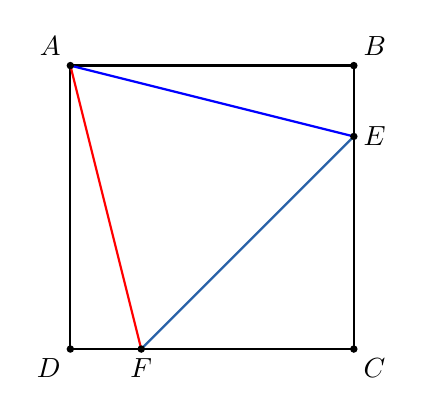
\begin{tikzpicture}[scale=0.9]
  \coordinate (A) at (0,4);
  \coordinate (B) at (4,4);
  \coordinate (C) at (4,0);
  \coordinate (D) at (0,0);
  \coordinate (E) at (4,3);
  \coordinate (F) at (1,0);
  \draw[thick] (A) -- (B) -- (C) -- (D) -- cycle;
  \draw[thick, blue] (A) -- (E);
  \draw[thick, red] (A) -- (F);
  \draw[thick, mainblue] (E) -- (F);
  \fill (A) circle (1.5pt) node[above left]{$A$};
  \fill (B) circle (1.5pt) node[above right]{$B$};
  \fill (C) circle (1.5pt) node[below right]{$C$};
  \fill (D) circle (1.5pt) node[below left]{$D$};
  \fill (E) circle (1.5pt) node[right]{$E$};
  \fill (F) circle (1.5pt) node[below]{$F$};
\end{tikzpicture}
\end{center}
\end{examplebox}

\textbf{证明：}

\begin{enumerate}[label=(\arabic*)]
  \item 将 $\triangle ABE$ 绕点 $A$ 逆时针旋转 $90°$ 得到 $\triangle ADF$。

  由旋转性质：
  \begin{itemize}[nosep]
    \item $AE = AF$（对应点到旋转中心距离相等）；
    \item $\angle EAF = 90°$（旋转角为 $90°$，即 $\angle EAF$ 等于旋转角）。
  \end{itemize}

  所以 $\triangle AEF$ 是等腰直角三角形。

  \item 由旋转知 $DF = BE = 1$，$AF = AE$。

  在 $\triangle ABE$ 中，$AB = 4$，$BE = 1$，$\angle B = 90°$：
  \[
  AE = \sqrt{AB^2 + BE^2} = \sqrt{16 + 1} = \sqrt{17}
  \]
  所以 $AF = AE = \sqrt{17}$。

  在等腰直角三角形 $AEF$ 中，斜边：
  \[
  EF = \sqrt{2} \cdot AE = \sqrt{2} \cdot \sqrt{17} = \sqrt{34}
  \]
\end{enumerate}

\begin{tipbox}[方法总结]
正方形中的旋转问题非常经典。绕正方形顶点旋转 $90°$ 时，对应点到顶点距离相等，且夹角为 $90°$，自然构造出等腰直角三角形。这类题的核心是利用旋转性质得到边等和角等的关系。
\end{tipbox}

\vspace{6pt}

\begin{examplebox}[【例题5】中心对称的判定与性质]
如图，平行四边形 $ABCD$ 的对角线 $AC$ 与 $BD$ 相交于点 $O$。求证：平行四边形 $ABCD$ 是中心对称图形，对称中心为 $O$。
\end{examplebox}

\textbf{证明：}

在平行四边形 $ABCD$ 中，对角线互相平分，即：
\[
OA = OC, \quad OB = OD
\]

将平行四边形 $ABCD$ 绕点 $O$ 旋转 $180°$：
\begin{itemize}[nosep]
  \item 点 $A$ 绕 $O$ 旋转 $180°$ 后，由于 $OA = OC$，$A$ 落在 $C$ 处。
  \item 点 $B$ 绕 $O$ 旋转 $180°$ 后，由于 $OB = OD$，$B$ 落在 $D$ 处。
  \item 同理，$C$ 落在 $A$ 处，$D$ 落在 $B$ 处。
\end{itemize}

旋转 $180°$ 后，$A \to C$，$B \to D$，$C \to A$，$D \to B$，四边形 $ABCD$ 与 $CDAB$ 重合，即与自身重合。

所以平行四边形 $ABCD$ 是中心对称图形，对称中心为对角线交点 $O$。

\begin{tipbox}[方法总结]
证明一个图形是中心对称图形，需要证明它绕某点旋转 $180°$ 后能与自身重合。平行四边形是中心对称图形，对称中心是对角线交点。这也解释了平行四边形对角线互相平分的几何意义。
\end{tipbox}

\vspace{6pt}

\begin{examplebox}[【例题6】综合题——旋转与坐标系]
在平面直角坐标系中，已知 $A(1,\, 2)$，$B(3,\, 1)$，$C(2,\, 4)$。
\begin{enumerate}[label=(\arabic*)]
  \item 求 $\triangle ABC$ 各顶点关于原点对称的点的坐标。
  \item 求 $A$ 点绕原点顺时针旋转 $90°$ 后的坐标。
\end{enumerate}
\end{examplebox}

\textbf{解：}
\begin{enumerate}[label=(\arabic*)]
  \item 关于原点对称，横纵坐标都变号：
  \[
  A(1,\, 2) \to A'(-1,\, -2), \quad B(3,\, 1) \to B'(-3,\, -1), \quad C(2,\, 4) \to C'(-2,\, -4)
  \]
  \item 顺时针旋转 $90°$ 的坐标变换：$(x,\, y) \to (y,\, -x)$。
  \[
  A(1,\, 2) \to A''(2,\, -1)
  \]
\end{enumerate}

\begin{tipbox}[方法总结]
坐标系中的对称与旋转问题，关键是熟记坐标变换公式。关于原点对称"双变号"，绕原点旋转 $90°$ "交换并变一个号"。
\end{tipbox}

% ==============================================================
% 第三部分：应用题
% ==============================================================
\section*{\textcolor{apppurple}{三、应用题}}

\begin{appbox}[【应用1】风车叶片的旋转]
一个风车有 $4$ 个叶片，每个叶片可以看作一个三角形。风车绕中心旋转，从起始位置到叶片转过 $270°$，风车转了多少圈？如果风车每分钟转 $60$ 圈，那么叶片转过 $270°$ 需要多少秒？
\end{appbox}

\textbf{解：}

$270° = \dfrac{270}{360}$ 圈 $= \dfrac{3}{4}$ 圈。

如果每分钟转 $60$ 圈，则每秒转 $1$ 圈。

转 $\dfrac{3}{4}$ 圈需要 $\dfrac{3}{4}$ 秒 $= 0.75$ 秒。

\begin{tipbox}[方法总结]
旋转角度与圈数的关系：$360°$ 对应一圈。实际问题中，将角度转化为圈数或分数圈是常见思路。
\end{tipbox}

\vspace{6pt}

\begin{appbox}[【应用2】机械臂的旋转定位]
工厂中一台机械臂绕固定点 $O$ 旋转工作。机械臂末端从位置 $A$ 顺时针旋转 $120°$ 到达位置 $B$，再从 $B$ 顺时针旋转 $90°$ 到达位置 $C$。若机械臂长 $OA = 2$ 米，求：
\begin{enumerate}[label=(\arabic*)]
  \item $A$ 到 $C$ 总共旋转了多少度？
  \item $OA$ 与 $OC$ 的夹角是多少度？
  \item $AC$ 的长度。（提示：$\angle AOC = 210°$，取 $360° - 210° = 150°$ 为较小夹角）
\end{enumerate}
\end{appbox}

\textbf{解：}
\begin{enumerate}[label=(\arabic*)]
  \item 总旋转角度 $= 120° + 90° = 210°$（均为顺时针）。
  \item $OA$ 与 $OC$ 的夹角 $= 210°$（取 $360° - 210° = 150°$ 为较小角）。
  \item 取 $\angle AOC = 150°$，$OA = OC = 2$。

  在 $\triangle AOC$ 中，由余弦定理：
  \[
  AC^2 = OA^2 + OC^2 - 2 \cdot OA \cdot OC \cdot \cos 150° = 4 + 4 - 2 \cdot 2 \cdot 2 \cdot \left(-\frac{\sqrt{3}}{2}\right) = 8 + 4\sqrt{3}
  \]
  \[
  AC = \sqrt{8 + 4\sqrt{3}} = 2\sqrt{2 + \sqrt{3}} \approx 2 \times 1.93 = 3.86 \text{（米）}
  \]
\end{enumerate}

\vspace{6pt}

\begin{appbox}[【应用3】瓷砖图案设计]
用旋转的方法设计地砖图案。取一个基本图形（如直角三角形），绕其中心依次旋转 $60°$，可以拼出正六边形图案。如果基本三角形的两条直角边分别为 $3$ cm 和 $4$ cm，求拼出的正六边形的面积。
\end{appbox}

\textbf{解：}

一个基本三角形的面积 $= \dfrac{1}{2} \times 3 \times 4 = 6$ cm$^2$。

绕中心旋转 $60°$ 共 $6$ 次，拼成 $6$ 个全等三角形组成正六边形。

正六边形面积 $= 6 \times 6 = 36$ cm$^2$。

\begin{tipbox}[方法总结]
旋转在图案设计中应用广泛。通过将基本图形绕中心旋转等角度（如 $60°$、$90°$、$120°$），可以拼出各种美丽的对称图案。
\end{tipbox}

% ==============================================================
% 第四部分：课堂练习
% ==============================================================
\section*{\textcolor{tipgreen}{四、课堂练习}}

\begin{enumerate}
  \item 点 $P(2,\, -3)$ 关于原点对称的点的坐标是\blank{3cm}。

  \item 将点 $A(1,\, 0)$ 绕原点逆时针旋转 $90°$ 后得到的点的坐标是\blank{3cm}。

  \item 如图，$\triangle OAB$ 绕点 $O$ 逆时针旋转 $60°$ 得到 $\triangle OCD$，$OA = 5$，$OB = 3$，求 $OC$、$OD$ 的长及 $\angle AOC$ 的度数。

  \item 判断正误：平行四边形是中心对称图形，也是轴对称图形。（\quad）

  \item 在正方形 $ABCD$ 中，$E$ 是 $CD$ 的中点，将 $\triangle ADE$ 绕点 $A$ 顺时针旋转 $90°$ 得到 $\triangle ABF$。若正方形边长为 $4$，求 $EF$ 的长。

  \item 已知 $A(3,\, 1)$，$B(5,\, 3)$，$C(1,\, 5)$，分别求出它们关于原点对称的点 $A'$、$B'$、$C'$ 的坐标，并判断 $\triangle ABC$ 与 $\triangle A'B'C'$ 的关系。
\end{enumerate}

\vspace{10pt}

\begin{knowledgebox}[参考答案]

\textbf{1.} $P'(-2,\, 3)$。关于原点对称，横纵坐标都变号。

\medskip
\textbf{2.} $(0,\, 1)$。$A(1,\, 0)$ 在 $x$ 轴正半轴上，绕原点逆时针旋转 $90°$ 后落在 $y$ 轴正半轴上，距原点仍为 $1$，所以坐标为 $(0,\, 1)$。

\medskip
\textbf{3.} $OC = OA = 5$，$OD = OB = 3$，$\angle AOC = 60°$（旋转角）。

\medskip
\textbf{4.} 错误。平行四边形是中心对称图形，但一般的平行四边形不是轴对称图形。只有特殊的平行四边形（长方形、正方形、菱形）才是轴对称图形。

\medskip
\textbf{5.} 由旋转知 $BF = DE = 2$，$AF = AE$。

在 $\triangle ADE$ 中，$AD = 4$，$DE = 2$，$\angle D = 90°$：

$AE = \sqrt{AD^2 + DE^2} = \sqrt{16 + 4} = \sqrt{20} = 2\sqrt{5}$。

$AF = AE = 2\sqrt{5}$，$\angle EAF = 90°$。

$EF = \sqrt{2} \cdot AE = 2\sqrt{5} \cdot \sqrt{2} = 2\sqrt{10}$。

\medskip
\textbf{6.} $A'(-3,\, -1)$，$B'(-5,\, -3)$，$C'(-1,\, -5)$。

$\triangle ABC$ 与 $\triangle A'B'C'$ 关于原点中心对称，因此全等。

\end{knowledgebox}

\vfill
\begin{center}
\small\textcolor{gray}{本讲义仅供教学参考，例题可根据学生水平调整难度。}
\end{center}

\end{document}
